% Pandoc template for docs/conclusions.tex (LuaLaTeX + biblatex/biber). Used by docs/build.sh.
\documentclass[11pt,a4paper]{article}
\usepackage[margin=2.6cm]{geometry}
\usepackage{fontspec}
\setmainfont{Libertinus Serif}
\setsansfont{Libertinus Sans}
\setmonofont{Libertinus Mono}[Scale=MatchLowercase]
\usepackage[french]{babel}
\usepackage{csquotes}
\usepackage{microtype}
\usepackage{xcolor}
\definecolor{link}{HTML}{0072B2}
\usepackage{graphicx}
\usepackage{longtable,booktabs,array,calc,etoolbox}
\makeatletter
\patchcmd\longtable{\par}{\if@noskipsec\mbox{}\fi\par}{}{}
\newsavebox\pandoc@box
\newcommand*\pandocbounded[1]{%
  \sbox\pandoc@box{#1}%
  \Gscale@div\@tempa{\textheight}{\dimexpr\ht\pandoc@box+\dp\pandoc@box\relax}%
  \Gscale@div\@tempb{\linewidth}{\wd\pandoc@box}%
  \ifdim\@tempb\p@<\@tempa\p@\let\@tempa\@tempb\fi
  \ifdim\@tempa\p@<\p@\scalebox{\@tempa}{\usebox\pandoc@box}\else\usebox{\pandoc@box}\fi}
\def\fps@figure{htbp}
\makeatother
\providecommand{\tightlist}{\setlength{\itemsep}{0pt}\setlength{\parskip}{0pt}}
\usepackage[font=small,labelfont=bf,labelsep=period]{caption}
\setlength{\parskip}{0.4em}
\setlength{\parindent}{0pt}
\setlength{\emergencystretch}{3em}
\usepackage[backend=biber,style=authoryear-comp,maxcitenames=2,uniquename=false,uniquelist=false,dashed=false]{biblatex}
\addbibresource{refs.bib}
\usepackage[hidelinks]{hyperref}
\hypersetup{colorlinks=true,linkcolor=link,citecolor=link,urlcolor=link,
  pdftitle={Survey, revisited},pdfauthor={Warith
Harchaoui},pdflang={fr}}
\IfFileExists{xurl.sty}{\usepackage{xurl}}{}

\title{\textbf{Survey, revisited}\\[0.4em]\large La grille de Pineau
(2018) réappliquée à la littérature de 2025-2026, puis à nos propres
expériences}
\author{Warith Harchaoui}
\date{9 novembre 2026 · état intermédiaire}

\begin{document}
\maketitle

\section*{Résumé}\label{ruxe9sumuxe9}
\addcontentsline{toc}{section}{Résumé}

En 2018, Joelle Pineau a passé 50 articles d'apprentissage par
renforcement (RL) au crible d'une grille de reproductibilité, et montré
avec Henderson et al.~qu'un même code, lancé avec deux graines, peut
ressembler à deux algorithmes
\autocite{pineau2018iclr,pineau2018neurips,henderson2018matters}. Notre
approche, \emph{survey, revisited}, refait ce travail sur deux plans.
D'abord le sondage : la même grille, appliquée à 50 articles tirés au
hasard parmi les 1 252 articles de RL d'ICLR 2026, d'ICML 2026 et de
NeurIPS 2025. Ensuite les expériences : celles de 2018, relancées avec
les algorithmes de 2026 et sous les règles que la grille réclame,
protocole écrit avant le premier entraînement.

Trois résultats sont acquis à ce jour. (1) L'évaluation tenue à part est
passée de 10 \% à 70 \% des articles, mais les hyperparamètres des
références ne sont plus donnés que dans 18 \% des articles (60 \% en
2018) et le test de significativité reste à 4 \%. (2) Sur 30 graines de
PPO, deux groupes de cinq tirés au hasard ne trompent le test de Welch
que dans 1,2 \% des cas ; ce qui trompe, c'est l'écart apparent (17 \%
en médiane), la coupe « cinq meilleures contre cinq pires » (31 \% de
faux positifs) et la sélection des trois meilleures sur dix (+33 \%).
(3) Notre propre référence « mal réglée » l'était d'abord par nous. Le
reste du programme (E2 à E5, E7, GRPO) est en cours ; ce document le dit
section par section.

\section{Introduction}\label{introduction}

La conférence invitée de Pineau à ICLR 2018 tient en une thèse : un
résultat n'est crédible que s'il est reproductible, et le RL profond ne
l'était pas \autocite{pineau2018iclr}. Elle s'appuyait sur deux mesures.
Un sondage de 50 articles, où environ 5 \% font un test de
significativité, et une série d'expériences sur MuJoCo
\autocite{todorov2012mujoco} où le classement des algorithmes change
d'une tâche à l'autre, où deux implémentations du même algorithme
divergent, et où deux paquets de cinq graines du même code TRPO
dessinent deux courbes séparées \autocite{henderson2018matters}.
L'argument rejoint celui de Buckheit et Donoho : un article est la
publicité de la recherche, pas la recherche
\autocite{buckheit1995wavelab}. Il s'inscrit dans une inquiétude plus
large, mesurée la même année par \emph{Nature}
\autocite{baker2016reproducibility}.

Depuis, la liste de contrôle de NeurIPS 2019, issue du programme qu'elle
a dirigé, est devenue la norme \autocite{pineau2021improving} ; les
statistiques du RL ont été revues \autocite{agarwal2021precipice} ; les
détails d'implémentation ont été mesurés
\autocite{engstrom2020implementation,andrychowicz2021matters}. Le RL a
aussi changé de terrain : il affine désormais de grands modèles de
langue à partir de récompenses vérifiables
\autocite{shao2024deepseekmath,deepseek2025r1}, et les mêmes pièges y
reparaissent. Une récompense tirée au sort y « marche » sur une famille
de modèles et pas sur les autres \autocite{shao2025spurious} ; le gain
en pass@1 peut se payer en pass@k \autocite{yue2025rlvr}.

\emph{Survey, revisited} pose donc deux questions. La grille de 2018
a-t-elle changé les pratiques ? Et nos propres expériences
survivent-elles aux règles que nous appliquons aux autres ?

\section{Méthode}\label{muxe9thode}

\subsection{Le sondage, refait}\label{le-sondage-refait}

Population : les 1 252 articles de RL d'ICLR 2026, d'ICML 2026 et de
NeurIPS 2025. Échantillon : 50 articles tirés au hasard (27 sur le RL de
grands modèles, 14 de RL classique, 9 de théorie dont 5 sans
expérience). Grille : celle de Pineau, complétée de quatre critères
qu'elle ne chiffrait pas (incertitude rapportée, références réglées
comme la méthode, calcul rapporté, sélection visible des meilleurs
essais). Calibration : 12 articles de RL d'ICML et de NeurIPS 2018, même
grille, mêmes lecteurs. Fidélité : deux lecteurs indépendants sur 10
articles s'accordent sur 127 décisions sur 130 (98 \%). Les parts sont
calculées sur les articles expérimentaux, avec l'intervalle de Wilson à
95 \% \autocite{wilson1927probable}. Protocole complet dans
\texttt{study/PROTOCOL.md}.

\subsection{Les expériences,
refaites}\label{les-expuxe9riences-refaites}

Le protocole \texttt{sim/SIM\_PROTOCOL.md} a été écrit le 8 novembre
2026, avant tout entraînement ; tout changement ultérieur est consigné
dans sa section « Écarts » avant d'avoir vu les résultats qu'il touche,
ou signalé comme postérieur. Outils figés : Gymnasium 1.1.1
\autocite{towers2024gymnasium}, MuJoCo, Stable-Baselines3 2.6.0
\autocite{raffin2021sb3} et sa version JAX. Algorithmes : PPO
\autocite{schulman2017ppo} en deux implémentations, SAC
\autocite{haarnoja2018sac} et CrossQ \autocite{bhatt2024crossq}. Tâches
: HalfCheetah, Hopper, Walker2d et Swimmer (\texttt{-v5}). Dix graines
par couple (algorithme, tâche), trente pour E1, aucune retirée.
Évaluation tenue à part : graines d'évaluation jamais vues à
l'entraînement, plus des dynamiques modifiées (masses × 1,2, frottement
× 0,8).

\begin{longtable}[]{@{}
  >{\raggedright\arraybackslash}p{(\linewidth - 4\tabcolsep) * \real{0.0658}}
  >{\raggedright\arraybackslash}p{(\linewidth - 4\tabcolsep) * \real{0.6184}}
  >{\raggedright\arraybackslash}p{(\linewidth - 4\tabcolsep) * \real{0.3158}}@{}}
\caption{Le programme expérimental et son état.}\tabularnewline
\toprule\noalign{}
\begin{minipage}[b]{\linewidth}\raggedright
Exp.
\end{minipage} & \begin{minipage}[b]{\linewidth}\raggedright
Question
\end{minipage} & \begin{minipage}[b]{\linewidth}\raggedright
État au 9 novembre
\end{minipage} \\
\midrule\noalign{}
\endfirsthead
\toprule\noalign{}
\begin{minipage}[b]{\linewidth}\raggedright
Exp.
\end{minipage} & \begin{minipage}[b]{\linewidth}\raggedright
Question
\end{minipage} & \begin{minipage}[b]{\linewidth}\raggedright
État au 9 novembre
\end{minipage} \\
\midrule\noalign{}
\endhead
\bottomrule\noalign{}
\endlastfoot
E1 & Deux groupes du même code ressemblent-ils à deux algorithmes ? &
fini, analysé \\
E2 & Le classement change-t-il d'une tâche à l'autre ? & en cours \\
E3 & Deux implémentations du même algorithme diffèrent-elles ? & en
cours \\
E4 & Que font les trois meilleurs essais sur dix ? & après E2 \\
E5 & Combien de graines pour retrouver le bon classement ? & après E2 \\
E6 & Que vaut une référence mal réglée ? & premier passage fini,
diagnostic en cours \\
E7 & Que perd-on hors des dynamiques d'entraînement ? & après E2 \\
\end{longtable}

\subsection{Le volet grands modèles}\label{le-volet-grands-moduxe8les}

GRPO \autocite{shao2024deepseekmath} écrit à la main, sur un portable
Apple, à petite échelle annoncée d'avance : Qwen2.5-0.5B-Instruct
\autocite{qwen2025qwen25} et Llama-3.2-1B-Instruct
\autocite{grattafiori2024llama3}, produit de deux nombres de 12 à 99,
vraie récompense contre récompense tirée au sort, comme Shao et al.
\autocite*{shao2025spurious}. Protocole :
\texttt{sim/llm/LLM\_PROTOCOL.md}.

\section{Résultats}\label{ruxe9sultats}

\subsection{Le sondage : ce qui a bougé, ce qui n'a pas
bougé}\label{le-sondage-ce-qui-a-bouguxe9-ce-qui-na-pas-bouguxe9}

\begin{figure}
\centering
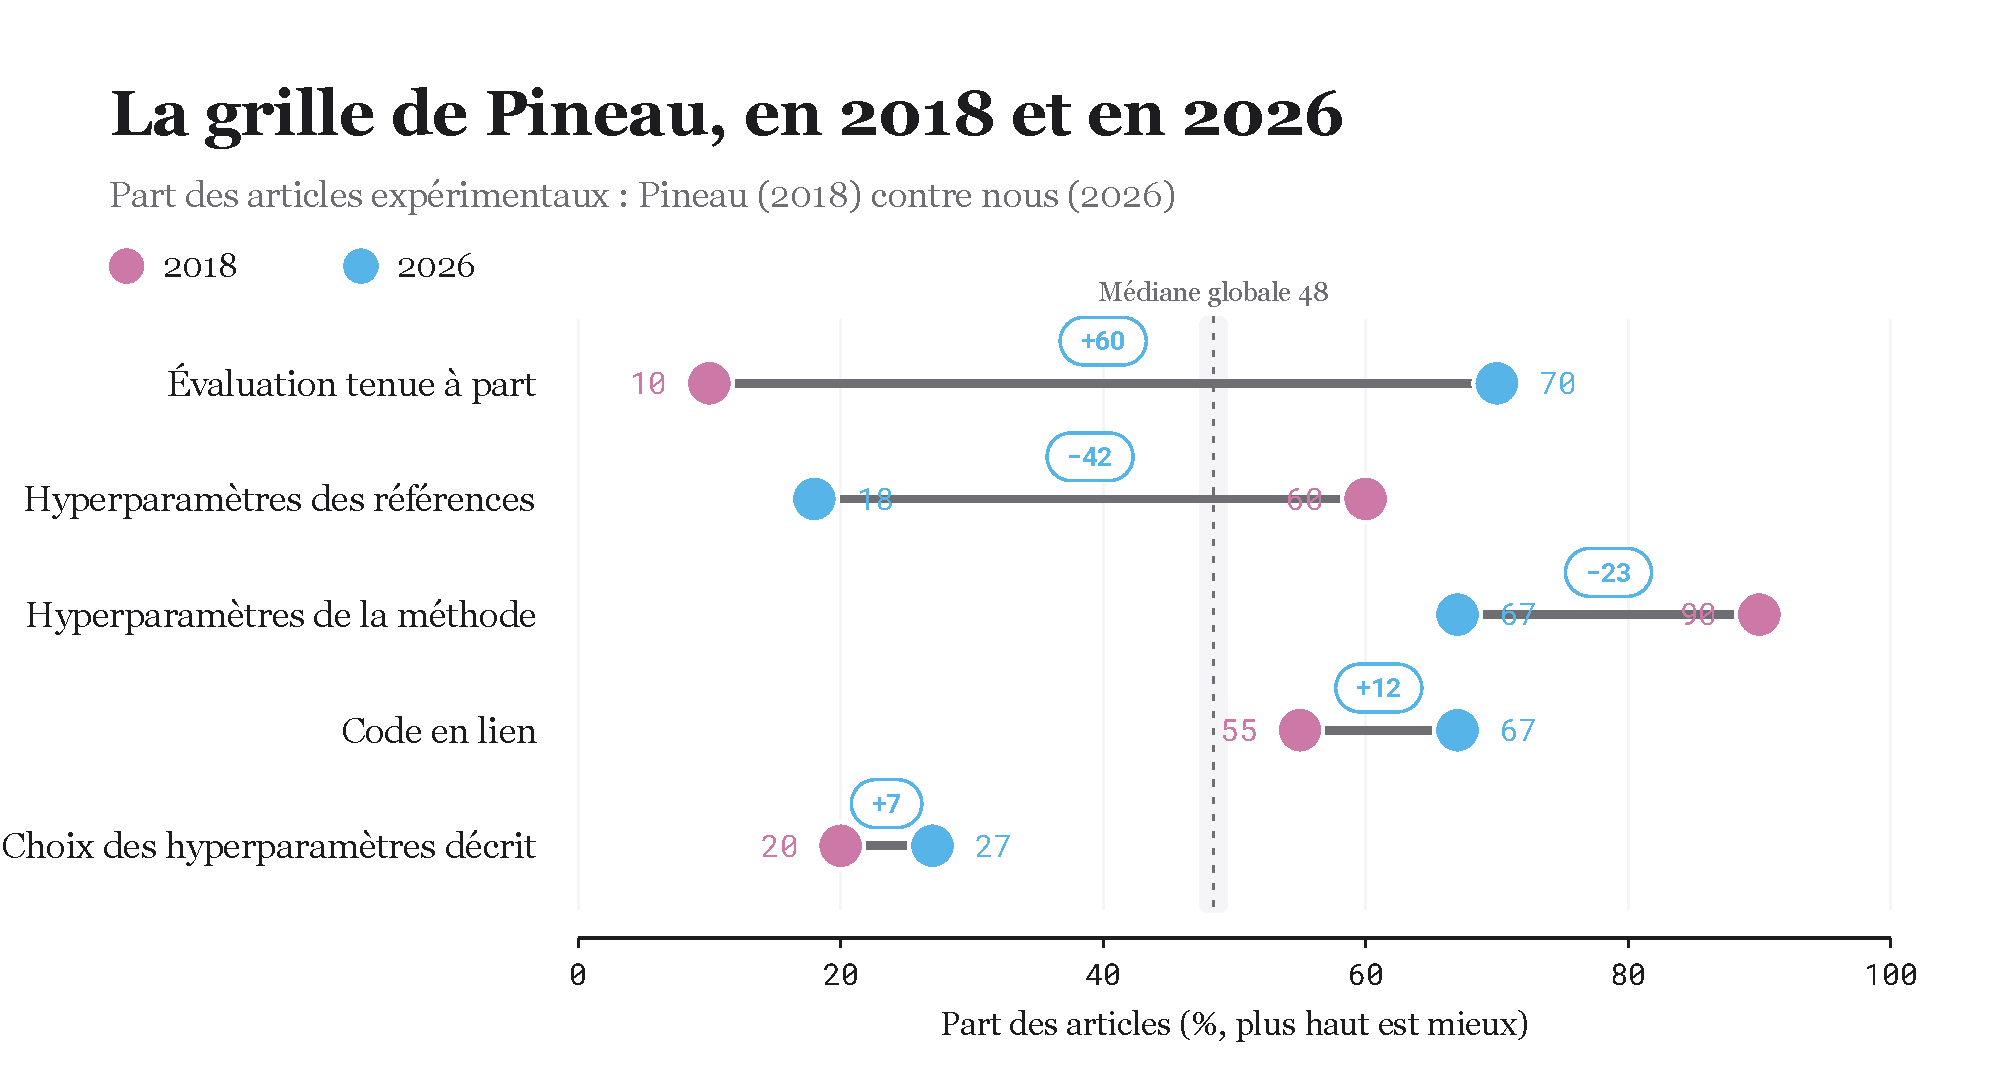
\includegraphics[width=1\linewidth,height=\textheight,keepaspectratio]{figures/remesure-dumbbell.pdf}
\caption{La grille de 2018 réappliquée. Points : part des articles
expérimentaux qui satisfont le critère, chez Pineau (2018) et dans notre
échantillon (2026). Le test de significativité, absent de la figure,
passe de 5 \% à 4 \%.}\label{fig:remesure}
\end{figure}

\begin{longtable}[]{@{}
  >{\raggedright\arraybackslash}p{(\linewidth - 6\tabcolsep) * \real{0.5211}}
  >{\raggedleft\arraybackslash}p{(\linewidth - 6\tabcolsep) * \real{0.1268}}
  >{\raggedleft\arraybackslash}p{(\linewidth - 6\tabcolsep) * \real{0.1549}}
  >{\raggedleft\arraybackslash}p{(\linewidth - 6\tabcolsep) * \real{0.1972}}@{}}
\caption{La grille de Pineau réappliquée. Données :
\texttt{study/results\_final.json}.}\tabularnewline
\toprule\noalign{}
\begin{minipage}[b]{\linewidth}\raggedright
Critère
\end{minipage} & \begin{minipage}[b]{\linewidth}\raggedleft
Pineau 2018
\end{minipage} & \begin{minipage}[b]{\linewidth}\raggedleft
Nous, calibration 2018
\end{minipage} & \begin{minipage}[b]{\linewidth}\raggedleft
Nous, 2026 {[}IC 95 \%{]}
\end{minipage} \\
\midrule\noalign{}
\endfirsthead
\toprule\noalign{}
\begin{minipage}[b]{\linewidth}\raggedright
Critère
\end{minipage} & \begin{minipage}[b]{\linewidth}\raggedleft
Pineau 2018
\end{minipage} & \begin{minipage}[b]{\linewidth}\raggedleft
Nous, calibration 2018
\end{minipage} & \begin{minipage}[b]{\linewidth}\raggedleft
Nous, 2026 {[}IC 95 \%{]}
\end{minipage} \\
\midrule\noalign{}
\endhead
\bottomrule\noalign{}
\endlastfoot
Hyperparamètres de la méthode, tous & 90 \% & 6/10 & 67 \% {[}52,
79{]} \\
Hyperparamètres des références, tous & 60 \% & 6/11 & \textbf{18 \%
{[}10, 32{]}} \\
Code en lien & 55 \% & 6/11 & 67 \% {[}52, 79{]} \\
Méthode de choix des hyperparamètres & 20 \% & 2/10 & 27 \% {[}16,
41{]} \\
Évaluation tenue à part & 10 \% & 4/10 & \textbf{70 \% {[}56, 82{]}} \\
Test de significativité & 5 \% & 1/11 & 4 \% {[}1, 15{]} \\
Incertitude rapportée & n.d. & 8/11 & 47 \% {[}33, 61{]} \\
Références réglées comme la méthode & n.d. & 4/10 & 5 \% {[}1, 15{]} \\
Calcul rapporté & n.d. & 4/11 & 47 \% {[}33, 61{]} \\
\end{longtable}

Un seul progrès net : l'évaluation tenue à part, portée par le RL de
grands modèles (26 articles sur 27, contre 5 sur 13 en RL classique).
Une régression nette : les hyperparamètres des références. Le reste n'a
pas bougé, test de significativité compris. L'incertitude rapportée
baisse, mais la baisse vient du RL de grands modèles (4 articles sur 27)
; le RL classique la rapporte toujours (14 sur 14).

\begin{figure}
\centering
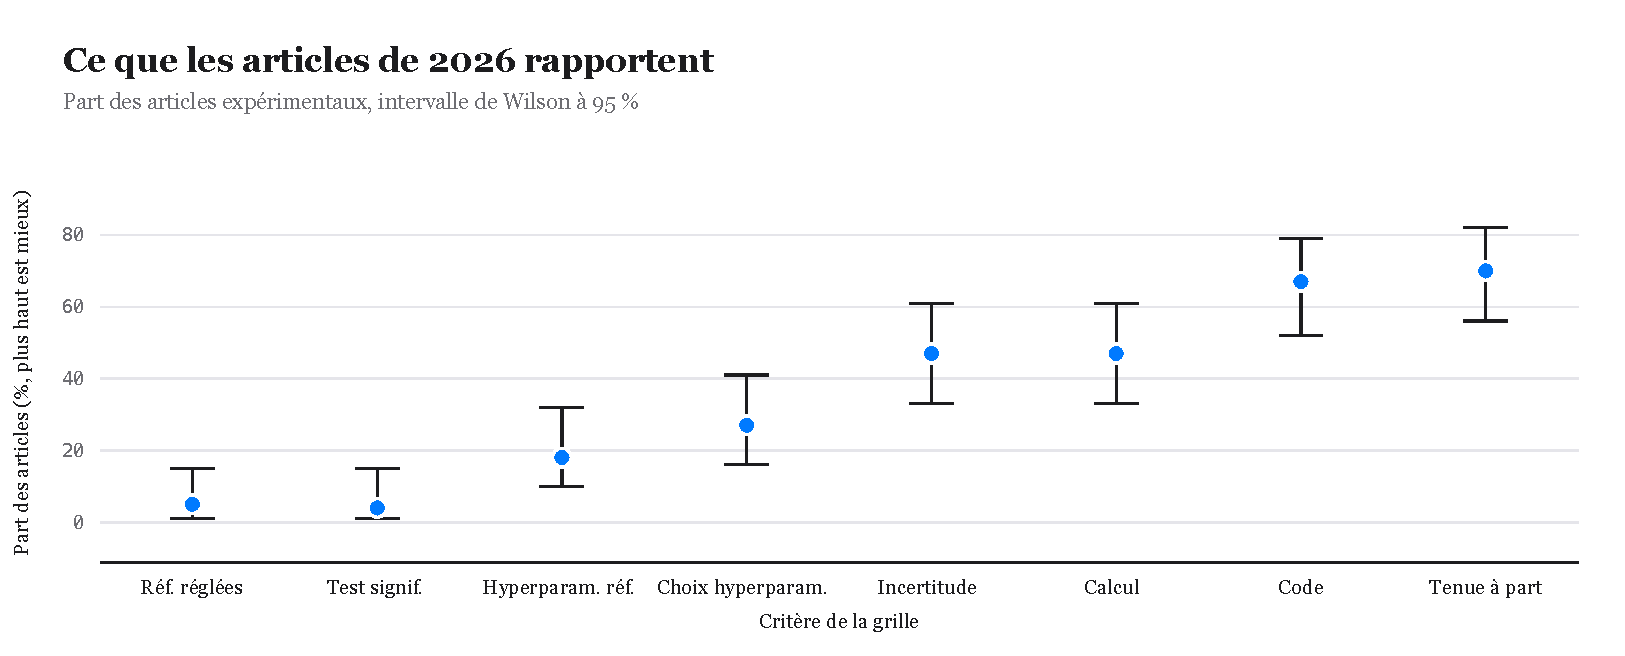
\includegraphics[width=1\linewidth,height=\textheight,keepaspectratio]{figures/remesure-ic.pdf}
\caption{Les critères de 2026 avec leur intervalle. Avec 45 articles
expérimentaux, un écart de moins de quinze points avec 2018 ne se
distingue pas du bruit d'échantillonnage.}\label{fig:remesure-ic}
\end{figure}

Graines : sur 41 articles de RL expérimentaux, 20 ne disent pas combien
d'entraînements indépendants soutiennent leurs résultats, 4 n'en ont
qu'un, et la médiane des autres est 5. En RL de grands modèles, 15
articles sur 27 n'essaient qu'une famille de modèles de base, alors que
Shao et al.~montrent qu'un effet peut ne valoir que pour une famille
\autocite*{shao2025spurious}.

\subsection{E1 : même code, autre
graine}\label{e1-muxeame-code-autre-graine}

\begin{figure}
\centering
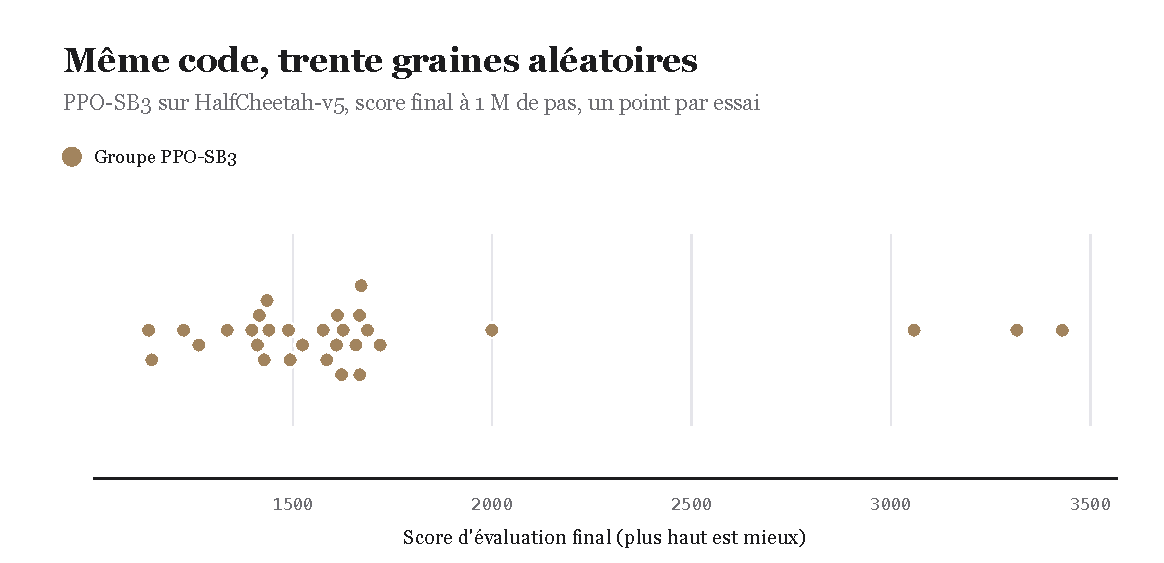
\includegraphics[width=1\linewidth,height=\textheight,keepaspectratio]{figures/e1-seeds.pdf}
\caption{Trente entraînements du même code, des mêmes hyperparamètres,
sur la même tâche ; seule la graine change. Moyenne 1 688, écart type
568 (coefficient de variation 34 \%), médiane 1 580.}\label{fig:e1}
\end{figure}

La distribution n'a rien de gaussien (Shapiro-Wilk, p = 4 ×
10\textsuperscript{−7}). Vingt-sept graines finissent entre 1 138 et 1
999 ; trois décollent au-delà de 3 000. Tirer cinq graines, c'est donc
tirer ou non l'une de ces trois-là.

\begin{figure}
\centering
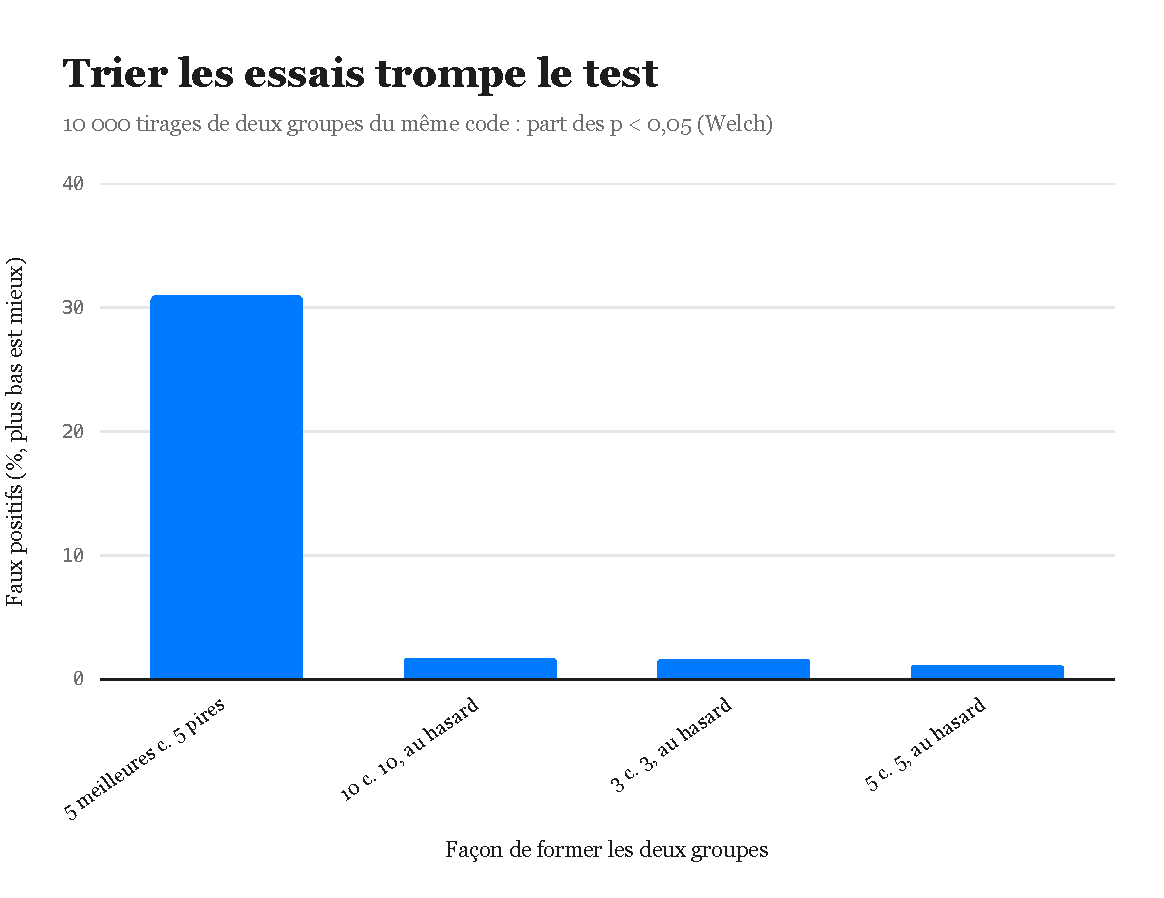
\includegraphics[width=0.9\linewidth,height=\textheight,keepaspectratio]{figures/e1-false-positive.pdf}
\caption{Part des 10 000 tirages où le test de Welch
\autocite{welch1947generalization} déclare différents deux groupes du
même code. Au hasard, le test est même prudent (1,2 \% à 1,7 \% pour un
seuil de 5 \%) ; la coupe triée le trompe une fois sur
trois.}\label{fig:e1-fp}
\end{figure}

\begin{longtable}[]{@{}
  >{\raggedright\arraybackslash}p{(\linewidth - 6\tabcolsep) * \real{0.5217}}
  >{\raggedleft\arraybackslash}p{(\linewidth - 6\tabcolsep) * \real{0.1594}}
  >{\raggedleft\arraybackslash}p{(\linewidth - 6\tabcolsep) * \real{0.1594}}
  >{\raggedleft\arraybackslash}p{(\linewidth - 6\tabcolsep) * \real{0.1594}}@{}}
\caption{E1, 10 000 tirages par ligne. Écart apparent : \textbar moyenne
A − moyenne B\textbar{} / min(moyennes). Données :
\texttt{sim/analysis/e1.json}.}\tabularnewline
\toprule\noalign{}
\begin{minipage}[b]{\linewidth}\raggedright
Façon de former les groupes
\end{minipage} & \begin{minipage}[b]{\linewidth}\raggedleft
Faux positifs (p \textless{} 0,05)
\end{minipage} & \begin{minipage}[b]{\linewidth}\raggedleft
Écart apparent médian
\end{minipage} & \begin{minipage}[b]{\linewidth}\raggedleft
95\textsuperscript{e} centile de l'écart
\end{minipage} \\
\midrule\noalign{}
\endfirsthead
\toprule\noalign{}
\begin{minipage}[b]{\linewidth}\raggedright
Façon de former les groupes
\end{minipage} & \begin{minipage}[b]{\linewidth}\raggedleft
Faux positifs (p \textless{} 0,05)
\end{minipage} & \begin{minipage}[b]{\linewidth}\raggedleft
Écart apparent médian
\end{minipage} & \begin{minipage}[b]{\linewidth}\raggedleft
95\textsuperscript{e} centile de l'écart
\end{minipage} \\
\midrule\noalign{}
\endhead
\bottomrule\noalign{}
\endlastfoot
3 contre 3, au hasard & 1,6 \% & 17 \% & 62 \% \\
5 contre 5, au hasard & 1,2 \% & 17 \% & 47 \% \\
10 contre 10, au hasard & 1,7 \% & 11 \% & 33 \% \\
5 meilleures contre 5 pires, sur 10 & 31,0 \% & 42 \% & --- \\
\end{longtable}

Ce résultat corrige notre propre lecture de 2018. Deux paquets de cinq
graines tirés au hasard ne trompent presque jamais un test ; ils
trompent l'œil. Un écart de 17 \% entre deux courbes est la norme sans
aucune différence d'algorithme, et un écart de 47 \% arrive une fois sur
vingt. Ce qui trompe le test, c'est la coupe triée de la figure de 2018
: 31 \% de faux positifs. La sélection trompe la moyenne : garder les
trois meilleures graines sur dix la gonfle de 33 \% (2 249 contre 1
692). Henderson et al.~rapportent t = −9,09 et p = 0,0016 entre deux
groupes de cinq ; leur légende précise que ce p est la moyenne des tests
faits le long de la courbe d'apprentissage, pas un test sur les scores
finaux, et l'article ne dit pas comment les dix essais ont été coupés en
deux \autocite{henderson2018matters}.

\subsection{E6 : la référence mal réglée, c'était
nous}\label{e6-la-ruxe9fuxe9rence-mal-ruxe9gluxe9e-cuxe9tait-nous}

E6 compare PPO sur Hopper avec les réglages par défaut de la
bibliothèque et avec les réglages publiés par RL Baselines3 Zoo
\autocite{raffin2020zoo}. Le premier passage donne au défaut une IQM de
2 877 {[}2 272, 3 346{]} et au Zoo 1 003 {[}859, 1 156{]}, le Zoo
plafonnant à 1 000 dès 50 000 pas. Ce résultat surprenant a déclenché
une vérification : notre normalisation des observations gardait γ = 0,99
là où le Zoo prend celui de l'algorithme, 0,999. La « référence mal
réglée » était d'abord la nôtre. Le premier passage est conservé tel
quel ; la recette corrigée a été relancée sur Hopper-v5 et v4 (la
version des réglages publiés), avec le défaut sur v4, dix graines
chacun. Ce diagnostic, ajouté après avoir vu le premier résultat, est
déclaré comme tel ; ses deux dernières graines tournent.

\subsection{GRPO : ce que mesurait vraiment la vraie
récompense}\label{grpo-ce-que-mesurait-vraiment-la-vraie-ruxe9compense}

Le pilote du taux d'apprentissage a été arrêté au pas 10 (65 Go de
mémoire, 29 Go de swap), sur une anomalie : 91 \% de réponses justes à
l'entraînement, contre 11 \% en pass@1 au test. Nous avons rejoué sans
entraînement le lot exact du pas 10 (48 × 49, 14 × 36, 21 × 50, 45 × 17)
avec le modèle de base.

\begin{figure}
\centering
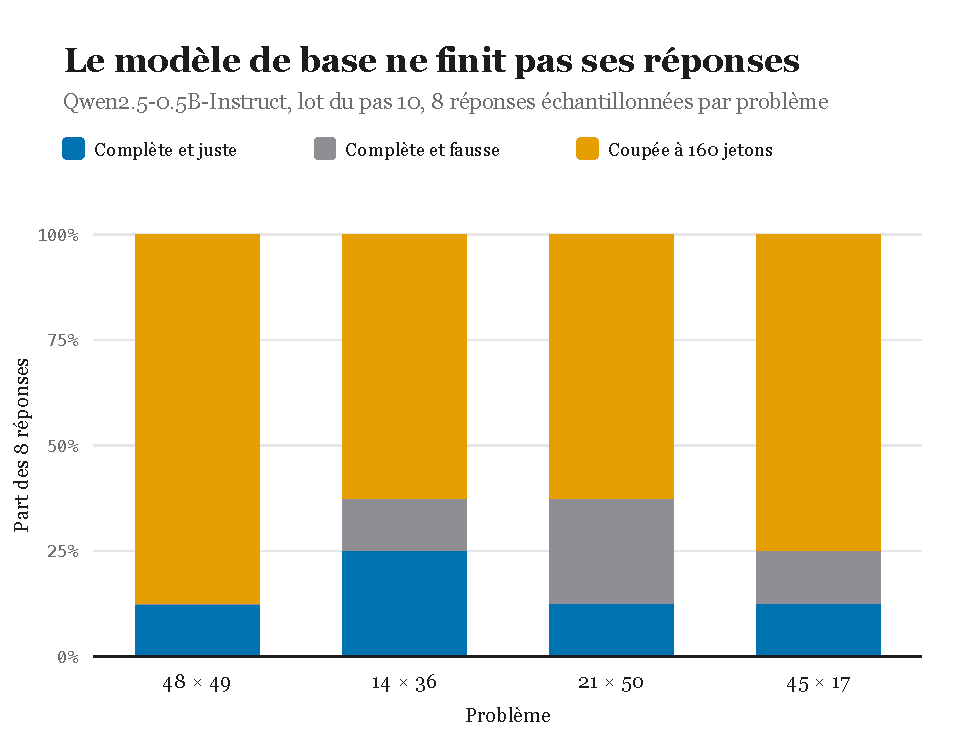
\includegraphics[width=0.8\linewidth,height=\textheight,keepaspectratio]{figures/grpo-truncation.pdf}
\caption{Le modèle de base sur le lot du pas 10. La plupart des réponses
atteignent la limite de 160 jetons avant de donner un
résultat.}\label{fig:grpo}
\end{figure}

Le modèle de base n'y fait que 5 sur 32, comme au test : le lot n'est
pas facile, et le décompte est juste. Mais 23 réponses sur 32 sont
coupées à 160 jetons, et aucune n'est juste ; parmi les 9 réponses
complètes, 5 le sont. Le faible score de départ mesure donc surtout la
longueur, et la vraie récompense apprend d'abord à finir avant la
coupure. La récompense tirée au sort n'a pas ce levier. Toute
comparaison entre les deux conditions doit séparer le gain de longueur
du gain d'arithmétique : la part de réponses coupées est désormais
mesurée à l'entraînement et au test. Une version réduite (100 pas, trois
graines, un entraînement à la fois, mémoire plafonnée) est lancée.

\section{Discussion}\label{discussion}

Huit ans après, la grille de Pineau a gagné une bataille, l'évaluation
tenue à part, et en a perdu une, la description des références. Le
progrès vient surtout du RL de grands modèles, dont les bancs d'essai
ont un jeu de test par construction ; d'où vient la régression, notre
échantillon ne permet pas de le dire. Le test de significativité, lui,
n'a jamais pris.

Nos expériences nuancent la figure la plus célèbre de 2018. Le hasard
des graines ne fabrique pas de faux positifs au rythme qu'on croit ; il
fabrique des écarts visibles, et ce sont nos choix (trier, garder les
meilleurs) qui les transforment en faux positifs. La règle utile n'est
donc pas seulement « plus de graines », mais « des graines qu'on ne trie
pas, et un intervalle plutôt qu'une courbe ». E5 dira combien.

Enfin, E6 et le diagnostic GRPO rappellent que la grille s'applique
d'abord à soi. Nous avons mal réglé la référence que nous voulions
montrer mal réglée, et notre premier indicateur GRPO mesurait une limite
de longueur. Les deux erreurs ont été trouvées parce que le protocole
était écrit d'avance et que les résultats surprenants ont été vérifiés
plutôt que publiés.

\section{Limites}\label{limites}

Le sondage porte sur 50 articles : les intervalles sont larges, et seuls
les écarts de plus de quinze points avec 2018 sont lisibles. Notre
calibration 2018 est plus sévère que la lecture de Pineau pour les
hyperparamètres de la méthode. E1 porte sur une seule tâche et un seul
algorithme. Le volet GRPO est une illustration sur des modèles de 0,5 et
1 milliard de paramètres, pas une réplication de Shao et al.

\section{Ce qui reste à mesurer}\label{ce-qui-reste-uxe0-mesurer}

E2 à E5 et E7 attendent la fin des simulations (environ 89
entraînements, 12 à 15 heures) ; E6 attend ses deux dernières graines ;
GRPO réduit tourne. Chaque expérience aura son script et son fichier
JSON dans \texttt{sim/analysis/}, et ce document sera mis à jour sans
retirer ce qui nous a contredits.

\section{Reproductibilité}\label{reproductibilituxe9}

Code, protocoles, journaux d'évaluation et scripts d'analyse :
\texttt{study/}, \texttt{sim/}, \texttt{sim/llm/}. Figures :
\texttt{docs/figures/build.py} les régénère toutes à partir des fichiers
de résultats. Environnement figé : \texttt{sim/requirements.lock}.

\printbibliography[title={Références}]
\end{document}
